\documentclass{article}
\usepackage{ctex}
\usepackage{tikz}
\usetikzlibrary{arrows.meta} % 引入一些箭头
\usetikzlibrary{calc} % 引入一些箭头
\usepackage{pgfplots} % 引入绘图宏包
\begin{document}


\section{箭头测试}

\begin{center}
    
    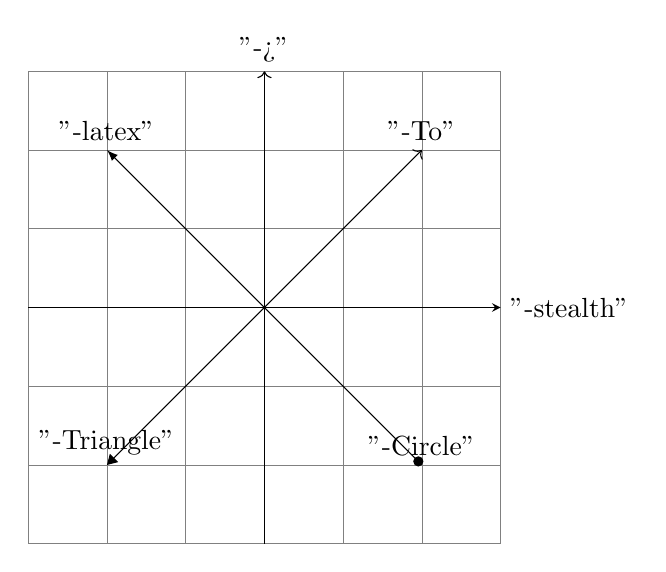
\begin{tikzpicture}
        \centering
        % 设置网格,方便观察坐标位置
        \draw[help lines] (-3,-3) grid (3,3);
        % 绘制 x 轴和 y 轴
        \draw[-stealth] (-3,0) -- (3,0) node[right] {"-stealth"};
        \draw[->] (0,-3) -- (0,3) node[above] {"->"};
        \draw[-To] (0,0) -- (2,2) node[above] {"-To"};
        
        \draw[-latex] (0,0) -- (-2,2) node[above] {"-latex"};
        
        %\usetikzlibrary{arrows.meta}
        \draw[-Triangle] (0,0) -- (-2,-2) node[above] {"-Triangle"};
        \draw[-Circle] (0,0) -- (2,-2) node[above] {"-Circle"};
    \end{tikzpicture}
    
\end{center}


\section{函数绘制}
\begin{figure}[h]
    \centering
    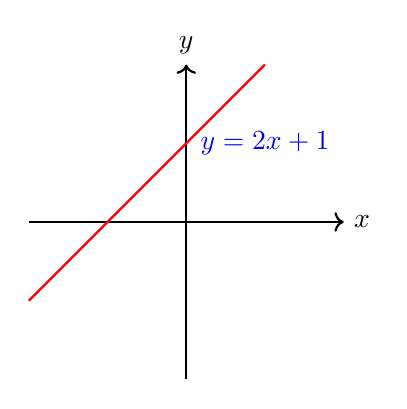
\begin{tikzpicture}[scale=1]
        % 绘制坐标轴
        \draw[->, thick] (-2,0) -- (2,0) node[right] {$x$};
        \draw[->, thick] (0,-2) -- (0,2) node[above] {$y$};
        % 绘制函数图像,添加 thick 选项使线条变粗
        \draw[domain=-2:1, smooth, variable=\x, red, thick] plot ({\x},{1*\x + 1});
        % 添加函数标签
        \node[blue] at (1,1) {$y = 2x + 1$};
    \end{tikzpicture}
    \caption{添加标题:类似图片的方法 }
\end{figure}



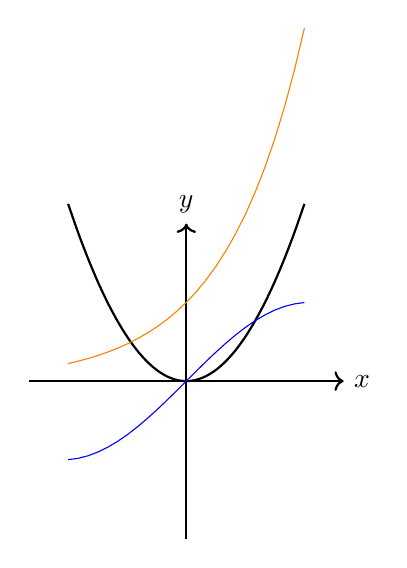
\begin{tikzpicture}[scale=1]
    % 绘制坐标轴
    \draw[->, thick] (-2,0) -- (2,0) node[right] {$x$};
    \draw[->, thick] (0,-2) -- (0,2) node[above] {$y$};
    % 绘制函数图像,添加 thick 选项使线条变粗
    \draw[domain=-1.5:1.5, smooth, variable=\x,  thick] plot ({\x},{\x*\x});
    % 添加函数标签
    \draw[domain=-1.5:1.5 ,color=blue] plot (\x,{sin(\x r)}); %r 表示弧度制

    \draw[domain=-1.5:1.5 ,color=orange] plot (\x,{exp(\x)}) ;
\end{tikzpicture}





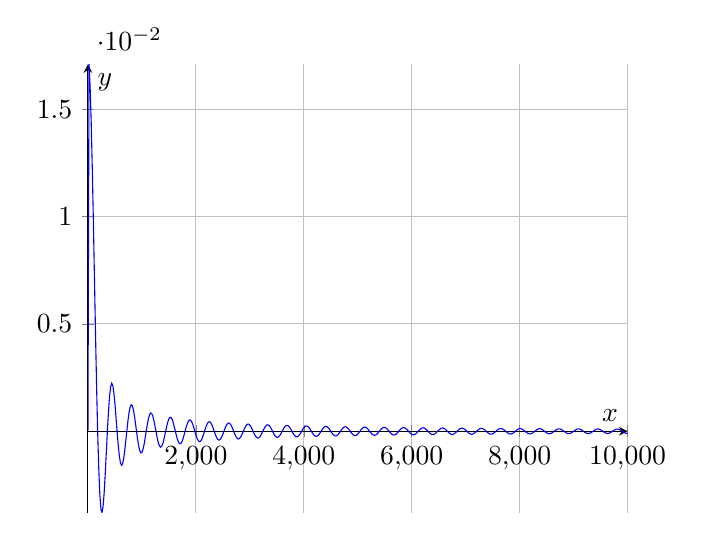
\begin{tikzpicture}[scale=1]
		\begin{axis}[
			axis lines =middle,
			xlabel = $x$,
			ylabel = {$y$},
			grid = major,
			]
			% 绘制函数 y = x^2
			\addplot [
			domain=0:10000, % 定义绘制区间
			samples=500, % 采样点数量,越高图像越平滑
			color=blue,
			]{(sin(x))/x };%基本上与数学环境中的函数差不多,去掉“\”就行了
		\end{axis}
	\end{tikzpicture}

\begin{tikzpicture}
		\begin{axis}[
			axis lines =middle,
			xlabel = $x$,
			ylabel = $y$,
			]
			\addplot [
			domain=-10:10, % 定义绘制区间
			samples=500, % 采样点数量,越高图像越平滑
			color=blue,
			]{(x*x) };%基本上与数学环境中的函数差不多,去掉“\”就行了
		\end{axis}
	\end{tikzpicture}




    \section{三角函数}
    \begin{tikzpicture}
        \begin{axis}[
            axis lines = middle,
            xlabel = $x$,
            ylabel = $y$,
            xmin = -2,
            xmax = 2,
            ymin = -2,
            ymax = 2,
            clip = false, % 设置不裁剪图形,也就是函数图像会超过坐标轴的范围
            axis line style={thick}, %使坐标轴变粗
            x axis line style={-Latex},
            y axis line style={-stealth},
            title = {取消刻度},   
            xtick=\empty,
            ytick=\empty %取消刻度
        ]
        \addplot [
            domain=-pi/2:pi/2 ,
            samples=500,
            color=blue
        ]{(sin(deg(x)))};
        \end{axis}
    \end{tikzpicture}
    \\
    \begin{tikzpicture}
        \begin{axis}[
            axis lines = middle,
            xlabel = $x$,
            ylabel = $y$,
            xmin = -3.5,
            xmax = 3.5,
            ymin = -2,
            ymax = 2,
            clip = false, % 设置不裁剪图形,也就是函数图像会超过坐标轴的范围
            axis line style={thick}, %使坐标轴变粗
            x axis line style={-Latex},
            y axis line style={-stealth},
            title = {设置$x$、$y$轴长度不同,但是图像上长度相同},   
            xtick=\empty,
            ytick=\empty %取消刻度
        ]
        \addplot [
            domain=-pi:pi ,
            samples=500,
            color=blue
        ]{(sin(deg(x)))};
        \end{axis}
    \end{tikzpicture}
    \\
    \begin{tikzpicture}
        \begin{axis}[
            axis lines = middle,
            xlabel = $x$,
            ylabel = $y$,
            xmin = -7,
            xmax = 7,
            ymin = -2,
            ymax = 2,
            clip = false, % 设置不裁剪图形,也就是函数图像会超过坐标轴的范围
            axis line style={thick}, %使坐标轴变粗
            x axis line style={-Latex},
            y axis line style={-stealth},
            title = {设置$x$、$y$轴长度不同,但是图像上长度相同},   
            xtick=\empty,
            ytick=\empty %取消刻度
        ]
        \addplot [
            domain=-2*pi:2*pi ,
            samples=500,
            color=blue
        ]{(sin(deg(x)))};
        \end{axis}
    \end{tikzpicture}

    \section{对数函数}
    \begin{tikzpicture}
        \begin{axis}[
            axis lines = middle, % 会影响x轴和y轴的相对位置
            xlabel = $x$,
            ylabel = $y$,
            xmin = -2,
            xmax = 2,
            ymin = -2,
            ymax = 2,
            clip = false, % 设置不裁剪图形,也就是函数图像会超过坐标轴的范围
            axis line style={thick}, %使坐标轴变粗
            x axis line style={-Latex},
            y axis line style={-stealth},
            title = {设置函数图像线宽:对数函数},   
            xtick=\empty,
            ytick=\empty %取消刻度
        ]
        \addplot [
            domain=0.1:pi/2 ,
            line width = 1.5pt,
            samples=500,
            % color=blue
        ]{(ln(x))};
        \end{axis}
    \end{tikzpicture}



    





\section{使用循环}

使用循环产生几个点\\

\begin{tikzpicture}
    % 语法:\foreach \变量 [选项] in {值列表} {命令}
    \foreach \x in {1,2,3,4,5} {
      \fill (\x, 0) circle (2pt);
    }
  \end{tikzpicture}
  


绘制几何图形\\
  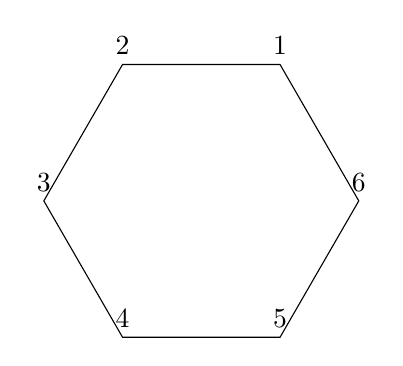
\begin{tikzpicture}
    % 绘制正六边形
    \def\n{6}  % 边数
    \def\r{2}  % 半径
    
    % 计算每个顶点的坐标
    \foreach \i in {1,...,\n} {
      \coordinate (P\i) at (\i*360/\n:\r);
    }
    % 连接所有顶点形成多边形
    \draw (P1) -- (P2) -- (P3) -- (P4) -- (P5) -- (P6) -- cycle;
    % 为每个顶点添加标签
    \foreach \i in {1,...,\n} {
      \node[above] at (P\i) {$\i$};
    }
  \end{tikzpicture}


  嵌套循环:绘制网格或矩阵\\
  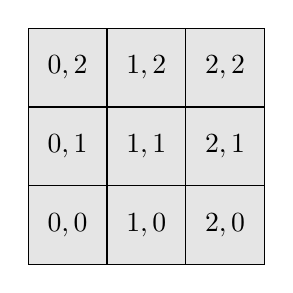
\begin{tikzpicture}
    % 绘制3×3网格
    \foreach \x in {0,1,2} {
      \foreach \y in {0,1,2} {
        \draw[fill=gray!20] (\x,\y) rectangle ++(1,1);
        \node at (\x+0.5,\y+0.5) {$\x,\y$};
      }
    }
  \end{tikzpicture}


  使用数学表达式生成序列\\
  \begin{tikzpicture}[scale=0.5]
    % 绘制f(x)=x²上的点
    \foreach \x in {-3,-2.5,...,3} {
      \fill[red] (\x, \x*\x) circle (2pt);
    }
  \end{tikzpicture}
  
  
  
  \begin{tikzpicture}[scale=0.5]
    \foreach \i in {-3,-2,-1,1,2,3} {
        \node at (\i,-0.2) {\i};
        \node at (-0.2,\i) {\i};
        }
  \end{tikzpicture}

  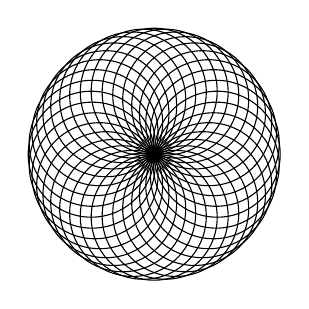
\begin{tikzpicture}[scale=0.8]
\foreach \i in {10,20,...,360} \draw (\i:1) circle (1);  %(\i:1) 表示 极坐标的圆心 (角度:半径)
  \end{tikzpicture}
  
  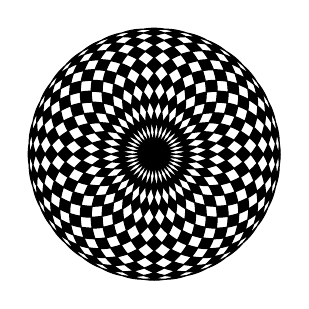
\begin{tikzpicture}[scale=0.8]
    \filldraw[even odd rule] \foreach \i in {10,20,...,360}
    {(\i:1) circle (1)};
  \end{tikzpicture}
  
  
  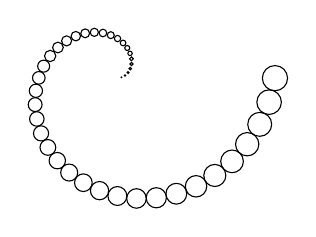
\begin{tikzpicture}[scale=2]
    \foreach \i in {0,0.025,...,1}
    \draw ($(0,0)!\i!\i*360:(1,0)$) circle(0.08*\i); %\i*360:(1,0) 将点 (1,0) 绕原点顺时针旋转 \i*360 度
  \end{tikzpicture}
  
  
  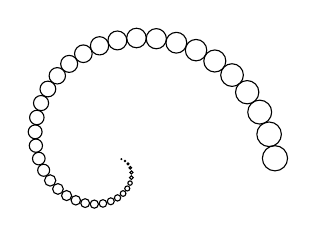
\begin{tikzpicture}[scale=2]
    \foreach \i in {0,0.025,...,1}
    \draw ($(0,0)!\i!-\i*360:(1,0)$) circle(0.08*\i); 
  \end{tikzpicture}
  
  \begin{center}
      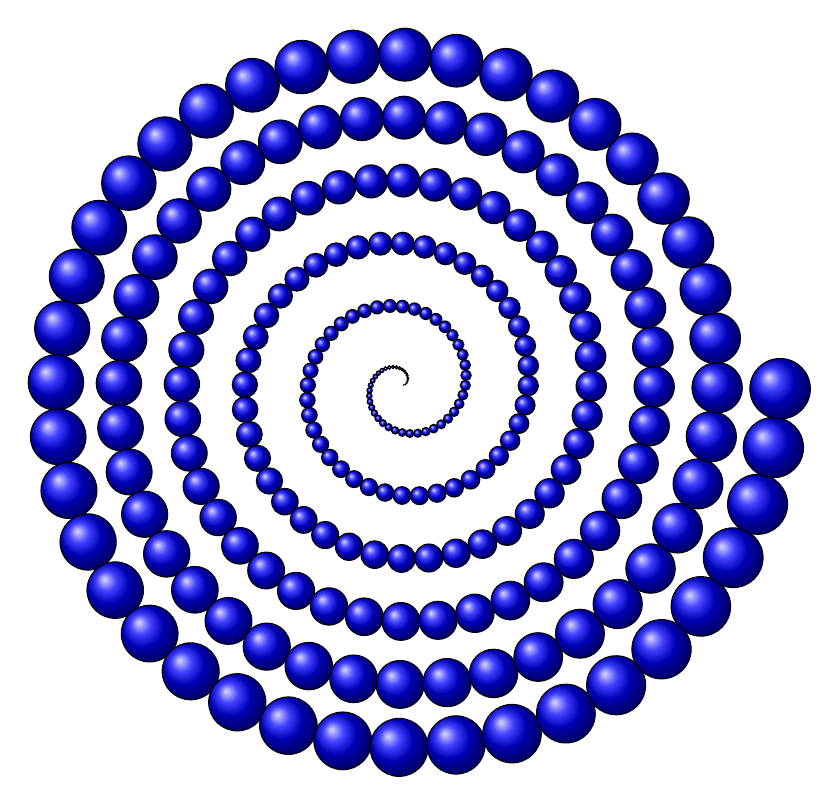
\begin{tikzpicture}[scale=0.8]
    \foreach \i in {0,0.025,...,6}
    \draw[shading=ball] ($(0,0)!\i!\i*360:(1,0)$)
    circle(0.08*\i);
  \end{tikzpicture}
  \end{center}

  
  \begin{center}
    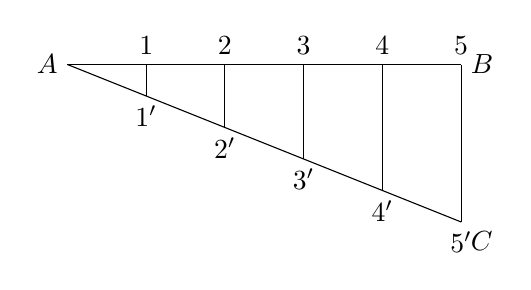
\begin{tikzpicture}[]
        % 标记点A, B, C
        \coordinate[label=left:{$A$}] (A) at (0,2);
        \coordinate[label=right:{$B$}] (B) at (5,2);
        \coordinate[label=below right:{$C$}] (C) at (5,0);

        % 绘制线段AB, AC
        \draw (A) -- (B);
        \draw (A) -- (C);

        % 等分线段AC
        \foreach \i in {1,...,5}
            {
                \coordinate[label=below:{$\i'$}] (a\i) at ($(A)!\i/5!(C)$);
                \coordinate[label=above:{$\i$}] (b\i) at ($(A)!\i/5!(B)$);
                \draw (a\i) -- (b\i);
            }

    \end{tikzpicture}
  \end{center}
\section{其他例子}


\begin{tikzpicture}[]

  \foreach \i in {0,0.025,...,1}
  \draw ($(0,0)!2!-\i*360:(1,0)$) circle(0.08*\i); 
\end{tikzpicture}







\end{document}
